
\documentclass[12pt]{article}
\usepackage{amsmath}
\usepackage{times}
\usepackage{graphicx}
\usepackage{color}
\usepackage{multirow}
%
\usepackage[authoryear]{natbib}
%
\usepackage{rotating}
\usepackage{bbm}
\usepackage{latexsym}
%\DeclareGraphicsExtensions{.eps,.png}

%%% margins 
\textheight 23.4cm
\textwidth 14.65cm
\oddsidemargin 0.375in
\evensidemargin 0.375in
\topmargin  -0.55in
%
\renewcommand{\baselinestretch}{2}
%
\interfootnotelinepenalty=10000
%
\renewcommand{\thesubsubsection}{\arabic{section}.\arabic{subsubsection}}
\newcommand{\myparagraph}[1]{\ \\{\em #1}.\ \ }
\newcommand{\citepaltt}[1]{\citepauthor{#1},\citepyear{#1}}
\newcommand{\myycite}[1]{\citepp{#1}}

% Different font in captions
\newcommand{\captionfonts}{\normalsize}

\makeatletter  
\long\def\@makecaption#1#2{%
  \vskip\abovecaptionskip
  \sbox\@tempboxa{{\captionfonts #1: #2}}%
  \ifdim \wd\@tempboxa >\hsize
    {\captionfonts #1: #2\par}
  \else
    \hbox to\hsize{\hfil\box\@tempboxa\hfil}%
  \fi
  \vskip\belowcaptionskip}
\makeatother   
%%%%%

\renewcommand{\thefootnote}{\normalsize \arabic{footnote}} 	


\newcommand{\ms}{\mbox{\,ms}}
\newcommand{\mV}{\mbox{\,mV}}
\newcommand{\s}{\mbox{\,s}}

\renewcommand{\u}{\mathbf{u}}
\renewcommand{\v}{\mathbf{v}}
\usepackage{amssymb}
\usepackage{tikz}
\usetikzlibrary{positioning}
\usetikzlibrary{arrows}

\begin{document}

\hspace{13.9cm}1

\ \vspace{20mm}\\

{\LARGE Calculating the Mutual Information Between Two Spike Trains}

\ \\
{\bf \large Conor Houghton$^{\displaystyle 1}$}\\
{$^{\displaystyle 1}$Computational Neuroscience Unit, Bristol University, England.}\\
%

%\ \\[-2mm]
{\bf Keywords:} Mutual information, electrophysiology data, Kozachenko-Loenenko

\thispagestyle{empty}
\markboth{}{Mutual information}
%
\ \vspace{-0mm}\\
%
%Abstract
\begin{center} {\bf Abstract} \end{center}
It is difficult to estimate the mutual information between spike
trains because established methods require more data than is usually
available. Kozachenko-Loenenko estimators promise to solve this
problem, but include a smooth parameter which must be set. It is
proposed here that the smoothing parameter can be selected by
maximizing the estimated unbiased mutual information. This is tested
on fictive data and shown to work very well.
%%%%%%%%%%%

\section{Introduction}

There are many problems in neuroscience that are addressed by
examining the relationship between the spiking output of two
neurons. The best way to do this should be to calculate the mutual
information between the two spike trains: the mutual information is a
measure of how much information the spike trains share and is
therefore an ideal way of quantifying the relationship between
them. However, in practice it has not been easy to use mutual
information in this way because of the huge amount of data required to
estimate it. This is because in the established method for calculating
information-theory quantities for spike trains, the spike trains are
converted into \lq{}words\rq{} by discretizing time; this produces a
huge number of words and so estimating their probabilities requires
more electrophysiological data than it is typically practical to
record.

In \citet{Houghton2015} a Kozachenko-Loenenko estimator
\citep{KozachenkoLeonenko1987,Victor2002,KraskovEtAl2004} is presented
for estimating the mutual information for random variables which take
values on a metric space, that is, for data where there are no
co\"{o}rdinates, but where it is possible to measure the distance
between two data points. This is relevant to the study of neuronal
data because there are many metrics on spike trains
\citep{VictorPurpura1996,vanRossum2001,AronovEtAl2003,HoughtonSen2008,HoughtonVictor2010}
which make the space of spike trains into a metric space.

This new method for calculating the mutual information between spike
trains relies on the choice of a smoothing parameter $h$. This paper
describes an effective way to select this parameter and tests this
method on fictive spike train data. It is found that the new method
produces the same result as the more traditional method, but does so
using considerably less spike train data.

The mutual information measures the dependence between two random
variables $U$ and $V$ and is given by
\begin{equation}
I(U;V)=\left\langle \log_2{\frac{p_{U,V}(\u,\v)}{p_U(\u)p_V(\v)}}\right\rangle
\end{equation}
where $\langle\ldots\rangle$ denotes the average with respect to the
joint distribution $p_{U,V}(\u,\v)$. $\u$ and $\v$ are values drawn
from the $U$ and $V$ variables respectively.  In the application
considered here the aim is to estimate the mutual information between
the activity of two neurons, so $\u$ and $\v$ are short intervals of
spike train, one from each of the two neurons; in this paper 45 ms
intervals are used. In order to calculate the mutual information the
probability mass function $p_{U,V}(\u,\v)$ needs to be estimated. The
method for calculating mutual information described here is
essentially a method of estimating the probability mass function.

The traditional method for calculating the mutual information is a
discretization method. For a bin width $\delta t$ each spike train
interval is converted into a word by binning the spikes and counting
the number of spikes in each bin. The mutual information is calculated
on the words rather than the spike trains with the probability of a
given word estimated by counting how often it occurs in the data. The
advantage of this method is that in the limit of vanishing $\delta t$
and of an infinite amount of data, the estimated mutual information
approaches the true value; the disadvantage is that it approaches this
true value very slowly. This is because of the huge number of words,
for example, with $45\ms$ long spike train intervals and $\delta
t=3\ms$ there are $2^{15}$ words and $2^{30}$, that is just over a
billion, pairs of words corresponding to the spike train pairs. This
situation can be improved with clever techniques
\citep{NemenmanEtAl2004,TrevesPanzeri1995} but one basic limitation is
that it considers each word individually. The power of a
Kozachenko-Loenenko approach is that is exploits the proximity
structure of a metric space meaning the data points are considered in
pairs.

Let $ \mathcal{P}=\{(\u_1,\v_1),(\u_2,\v_2),\ldots,(\u_n,\v_n)\} $
denote a set of pairs of intevals from spike trains recorded during an
experiment. These are modelled as being drawn from the probability
distribution $p_{U,V}(\u,\v)$. Following the formulation of the
Kozachenko-Loenenko estimator given in \citet{Houghton2015} this
probability distribution is approximated by
\begin{equation}
 p_{U,V}(\u_i,\v_i)\approx\frac{\#B}{\mbox{vol}\,(B)}
\end{equation}
where $B$ is a ball around the point $(\u_i,\v_i)$, $\#B$ is the number of
points in the ball and $\mbox{vol}(V)$ is the volume of the ball. This
approximation comes straight from the definition of the probability mass function
\begin{equation}
\left\langle \#B\right\rangle = \int_B p_{U,V}(\u,\v)dV
\end{equation}
with the addition assumption that $p_{U,V}(\u,\v)$ is approximately
contant on $B$. The idea is that for every point a ball of fixed
volume is used to estimate the probability mass function at that
point. The volume chosen for this ball is a smoothing parameter: the
larger the volume the more accurately $\#B$ estimates $\left\langle
\#B\right\rangle$, but for larger volumes the assumption that
$p_{U,V}(\u,\v)$ is approximately constant on $B$ becomes less
accurate.

The difficulty is how to calculate the volume of $B$. Because there
are no co\"{o}rdinates for the space of spike trains there is no
$dxdydz$-style integration measure. However, a probability
mass function does provide a volume measure on a space and as
described in detail in \citet{Houghton2015} the marginalized
distribution $p_U(\u)p_V(\v)$ can be used to provide a volume measure
on the space of spike train pairs.

Though this seems an odd choice of volume measure it gives a simple
formula for the mutual information. For a point $(u_i,v_i)$ consider
the nearest $h$ $U$-spike-train intervals to $u_i$:
\begin{equation}
C_U(\u_i,\v_i)=\{(\u_j,\v_j): d(\u_j,\u_i)\mbox{ is one of the }h\mbox{ smallest $U$-distances} \}
\end{equation}
and the nearest $h$ $V$-spike-train itervals to $v_i$
\begin{equation}
C_V(\u_i,\v_i)=\{(\u_j,\v_j): d(\v_i,\v_j)\mbox{ is one of the }h\mbox{ smallest $V$-distances}\}.
\end{equation}
Now the ball around $(\u_i,\v_i)$ is defined as
\begin{equation}
C(\u_i,\v_i)=C_U(\u_i,\v_i)\cup C_V(\u_i,\v_i)
\end{equation}
which has estimated volume $h^2/N^2$. Finally let $\#C(u_i,v_i)$ be the
number of $(u_j,v_j)$ points in $C(\u_i,\v_j)$:
\begin{equation}
\#C(u_i,v_i)=\#[C_U(\u_i,\v_i)\cap C_V(\u_i,\v_i)]
\end{equation}
With this notation the  Kozachenko-Loenenko approximation for the mutual information is given
\begin{equation}
I(U;V)\approx I_{\text{KL}}(\mathcal{P};h)=\frac{1}{n}\sum_{i=1}^n\log_2{\frac{n\#[C(u_i,v_i)]}{h^2}}
\end{equation}

This quantity is straightforward to calculate. For each point
$(\u_i,\v_i)$, the set $C_U(\u_i,\v_i)$ contains $(\u_i,\v_i)$ itself
and the nearest $h-1$ points to $(\u_i,\v_i)$ when $\u_i$ is compared
to the $\u_j$ in other $(\u_j,\v_j)$ pairs. Similarly, the set
$C_V(\u_i,\v_i)$ contains the nearest $h-1$ points when $\v_i$ is
compared to $v_j$. $\#C(\u_i,\v_i)$ is the size of the
intersection. This is illustrated in Fig.~\ref{fig_region}.

\begin{figure}
\begin{center}

  \setlength{\unitlength}{0.0500bp}%
  \begin{picture}(5040.00,3528.00)%
      \put(855,1818){\rotatebox{-270}{\makebox(0,0){\strut{}$V$}}}%
      \put(2519,154){\makebox(0,0){\strut{}$U$}}%
      \put(2400,3600){\makebox(0,0)[l]{\strut{}$C_U$}}%
      \put(4200, 1675){\makebox(0,0)[l]{\strut{}$C_V$}}%
      \put(2250,3400){\makebox(0,0)[l]{\strut{}$\overbrace{\;\,\qquad}$}}
      \put(3950,1665){\makebox(0,0)[l]{\strut{}$\left.\rule{0cm}{0.9cm}\right\}$}}
    \put(0,0){\includegraphics{region.eps}}%
  \end{picture}%


\end{center}
\caption{The calculation of $I_{\text{KL}}(\mathcal{P};h)$. The
  $U$-space corresponds to the horizonal direction, the $V$-space to
  the vertical, of course, this is a cartoon, these spaces are not
  one-dimensional, they do not even have a defined dimension. The
  points in $\mathcal{P}$ are marked as filled circles and a square;
  the square point is the one whose contribution to
  $I_{\text{KL}}(\mathcal{P};h)$ is being calculated. The grey bars
  represent $C_U(\blacksquare)$ and $C_V(\blacksquare)$ with $h=8$.
  $\#C(\blacksquare)=4$ since it counts the points in the
  intersection, that is, the region with darker
  shading.\label{fig_region}}
\end{figure}

It is instructive to consider what happens if the two distibutions are
independent. In this case the it is possible to calculate the
probability that $\#C(\u_i,\v_i)=r$ for different possible values $r$;
it is a sort of urn problem. Choosing the $h-1$ points in $C_U(\u_i,\v_i)$ that are not $(\u_i,\v_i)$ itself
is like randomly selecting $h-1$ points out of $n-1$ and calculating $r$ is ask how many
are in $C_V(\u_i,\v_i)$; this gives
%\begin{equation}
%\mbox{prob}\left(\#C(\u_i,\v_i)=r\right)=\frac{\left(\begin{array}{c}h\\r\end{array}\right)
%\left(\begin{array}{c}n-h\\h-r\end{array}\right)}{\left(\begin{array}{c}n\\h\end{array}\right)}
%\end{equation}
\begin{equation}
\mbox{prob}\left(\#C(\u_i,\v_i)=r\right)=\frac{\left(\begin{array}{c}h-1\\r-1\end{array}\right)
\left(\begin{array}{c}n-h\\h-r\end{array}\right)}{\left(\begin{array}{c}n-1\\h-1\end{array}\right)}
\end{equation}
so
\begin{equation}
I_0(n,h)=\sum_{r=1}^h \mbox{prob}\left(\#C(\u_i,\v_i)=r\right) \log_2{\frac{nr}{h^2}}
\end{equation}
is the estimated mutual information when the two distributions are
independent. This is a upward bias in the estimate of the mutual
information; an upward bias is a common feature of estimators of
mutual information. In this case the bias is because $B$ will not
always contain exactly $\langle \#B\rangle$ points. One advantage of
the Kozachenko-Loenenko approach is that $I_0$ gives an explicit
formula for the bias and it depends only on the smoothing parameter
$h$ and the number of pairs, $n$.

Obviously, as $h$ approachs $n$, this bias approaches zero but
otherwise it is positive and as bias it can be removed from the
estimate of the mutual information:
\begin{equation}
I(U;V)\approx\tilde{I}(\mathcal{P};h)=I_{\text{KL}}(\mathcal{P};h)-I_0(n,h)
\end{equation}
Recall that there are two competing approximations used in deriving
the estimate: for small $h$ the counting estimates for the number of
points in a ball and for the volume of the balls are noisy; for large
$h$ the estimate of the probability mass function is too smooth. The
first of these approximations is the cause of the bias described by
$I_0(n,h)$. Conversely $I_0(n,h)$ is not effected by the smoothing
bias. This suggests that the best approximation is found by maximizing
$\tilde{I}(\mathcal{P};h)$ over $h$:
\begin{equation}
I(U;V)\approx\tilde{I}(\mathcal{P})=\max_h{\tilde{I}(\mathcal{P};h)}
\end{equation}
It is demonstrated here that this works very well.

\section{Methods}

\subsection{Data}


\begin{figure}
\begin{center}
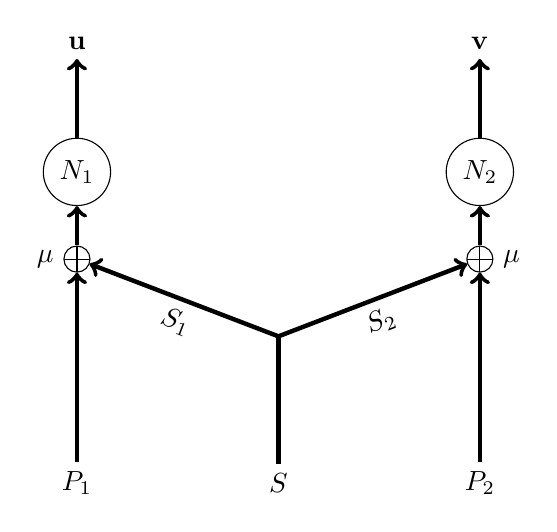
\begin{tikzpicture}[cross/.style={path picture={ 
  \draw[black] (path picture bounding box.south) -- (path picture
  bounding box.north) (path picture bounding box.west) -- (path
  picture bounding box.east); }}] \node (neuron1) at (0,0)
  [circle,draw] {$N_1$}; \node (middle)[right = 2cm of neuron1]{};
  \node (neuron2) [circle, right = 2cm of middle,draw] {$N_2$}; \node
  (a)[below = 1.5cm of neuron1]{}; \node (b)[below = 1.84cm of
    middle]{}; \node (c)[below = 1.5cm of neuron2]{};

\node (mu1)[circle,cross,below  = 0.5cm of neuron1,draw]{};
\node (mu2)[circle,cross,below  = 0.5cm of neuron2,draw]{};
\node (mumu1)[left = 0.0cm of mu1]{$\mu$};
\node (mumu2)[right = 0.0cm of mu2]{$\mu$};


\draw [ultra thick,->] (mu1)--(neuron1);
\draw [ultra thick,->] (mu2)--(neuron2);


\draw [ultra thick,->](b.center)--(mu1) node(s1)[midway, below, sloped]{$S_1$};
\draw [ultra thick,->](b.center)--(mu2) node(s2)[midway, below, sloped]{$S_2$};
\node(p1) [below=1.5cm of a]{$P_1$};
\node(s) [below=1.5cm of b]{$S$};
\node(p2) [below=1.5cm of c]{$P_2$};
\draw [ultra thick,->] (p1)--(mu1);
\draw [ultra thick](s)--(b.center);
\draw [ultra thick,->](p2)--(mu2);
\node (u) [above = 1cm of neuron1]{$\u$};
\node (v) [above = 1cm of neuron2]{$\v$};
\draw [ultra thick,->](neuron1)--(u);
\draw [ultra thick,->](neuron2)--(v);

\end{tikzpicture}
\end{center}
\caption{The fictive data. This shows the network used to produce the
  fictive data used to test the new formula for mutual
  information. $N_1$ and $N_2$ are both leaky integrate-and-fire
  neurons, producing the spike trains $\u$ and $\v$
  respectively. Their input is a weighted average of $P_i$ and $S_i$;
  $S$ is a shared input with $S_1=S$ and
  $S_2=\bar{S}-S$.\label{fig_network}}
\end{figure}

The algorithm is run on fictive data generated using two leaky
integrate-and-fire neurons with shared input; the two neurons satisfy
\begin{equation}
\tau_m \frac{dv_i}{dt}=E_l-v_i+I_i
\end{equation}
where, $i=1,2$ labels the two neurons, $\tau_m=12\ms$ and
$E_l=-70\mV$. If $v_i>V_t$, where $V_t=-70\mV$ a spike is recorded and
$v_i$ is reset to $E_l$; there is a refractory period of
$\tau_r=2\ms$. $I_i$ is an input, because the membrane resistance has
been absorbed into $I_i$ it is a voltage rather than a current. Here
\begin{equation}
I_i=\mu P_i +(1-\mu) S_i
\end{equation}
where $P_i$ is an input particular to the $i$ neuron whereas $S_i$ is an
input based on a shared input $S$:
\begin{eqnarray}
S_1&=&S\cr
S_2&=&\bar{S}-S
\end{eqnarray}
with $\bar{S}=30\mV$.  The inputs $P_i$ and $S$ are both piecewise
constant, with each having a fixed value for a period chosen
independently from a exponential distribution with mean
$\tau_c=30\ms$; the value for each interval is chosen uniformly from
$[0,\bar{S}]$. This network is illustrated in Fig.~\ref{fig_network}.

This method is not perfect in the sense that the temporal correlation
is different for different values of $\mu$ and the firing rate varies
from 63 Hz at $\mu=0$ and $\mu=1$, to 52 Hz at $\mu=0.5$. However, the
aim is to test the spike train pairs with different values of mutual
information and, as we shall see, this method does succeed in doing
that.

\subsection{The distance between spike trains}

For the new information calculation the distance between individual
spike trains is calculated using the van Rossum metric
\citep{vanRossum2001}, this calculates the distance between two spike
trains $\u=(u_1,u_2,\ldots,u_n)$ and
$\v=(v_1,v_2,\ldots,v_m)$ as
\begin{equation}
d(\u,\v)=\sum_{i,j} e^{-|u_i-u_j|/\tau}+\sum_{i,j} e^{-|v_i-v_j|/\tau}-2\sum_{i,j} e^{-|-u_i-v_i|/\tau}
\end{equation}
where $\tau$ is a timescale which can be thought of as expressing the
persicion of spike times in neuronal coding. A value around
$\tau=15\ms$ is often used. In the formula for mutual information the
metric is used to order points by proximity so it might be expected
that the values of estimated mutual information would not depend in a
detailed way on the distance values or on the choice of metric. In
fact, it will be seen here that in this application the results are
not sensitive to the value of $\tau$.

\subsection{Calculating the information}

The pairs spike trains produced by the network model are chopped up
into 45 ms intervals. To calculate the mutual information using the
\lq{}old\rq{} method these intervals are discritised with $\delta
t=3\ms$ giving 15 letter words. The frequency for each word pair is
estimated from the data using the obvious empirical estimate
\begin{equation}
p_{U,V}(\u,\v)\approx \frac{\mbox{occurances of }(\u,\v)}{\mbox{total number of samples}}.
\end{equation}
This is then used to calculate the mutual information directly. The
bias is removed by also calculating the mutual information for
shuffled data.

To calculate the mutual information using the \lq{}new\rq{} method,
the distance matrix for the $U$-spike trains and the $V$-spike trains
were calculated using the efficient implementation of the van Rossum
metric described in \citep{HoughtonKreuz2012}. The optimal value of $h$
was found using a golden mean search \citep{Kiefer1953}.

\section{Results}

In Fig.~\ref{fig_mu_sweep} the value of the mutual information for
$45\ms$ intervals of spike train is calculated for different values of
$\mu\in[0,1]$ using both the old and new approach. For the new
  approach $200\s$ of data is used; for the traditional method
  $25000\s$ of data is used to establish the ground truth and smaller
  value of $2000\s$ to illustrate the amount of data needed to
  estimate the mutual information.

\begin{figure}[tp]
\begin{center}
\include{fig_mu_sweep}
\end{center}
\caption{Estimates of the mutual information for different values of
  $\mu$. The mutual information between pairs of 45 ms fragments of
  spike train is estimated using the new and old approaches. In the
  case of the new approach 200 s of spike train is used, in the old
  approach, 2000 s and 25000 s are used. In all cases the graph shows
  the average of 100 trials; in the new approach $\tau=15\ms$, in the
  old approach 3 ms bins are used.\label{fig_mu_sweep}}
\end{figure}

Using 2000 s of data the old method gives a very poor estimate of the
mutual information for most values of $\mu$; the new method is much
closer to the value estimated using 25000 s of data. The old method
is better for values of $\mu>0.6$ when the amount of mutual
information is very low; presumably this is because the noise in the
estimate is more signicant and the maximization over $h$ leads to an
over-estimate.

Fig.~\ref{fig_length_sweep}\textbf{A} and \textbf{B} show the
convergence of the new and old estimates. This again shows that the
new method uses considerably less data than the old method. It is
clear from these graphs that the estimators approach their asymptotic
values in an orderly way. This means one approach to improving the
estimate using the old method is to fit the graph to a curve such as
\begin{equation}
I(a,b,c)=a+\frac{b}{\sqrt{T}}+\frac{c}{T\sqrt{T}}
\end{equation}
where $T$ is the length of spike train used. In the example being
examined here this works quite well, fixing $a$, $b$ and $c$ using the
first $2000$ s, gives an estimate of $0.6613$ for $T=25000\s$,
compared to an actual value of $0.7156$; the value given by new method
using 400 s of data is $0.7412$. The old method gives even larger
value if is even larger amounts of data were used, for this value of
$\mu$ 1000000 s of data gives 0.768413. Extrapolating the old method
from 200 s of data does not work, it gives an estimate of
$0.1975$. Fig.~\ref{fig_length_sweep}\textbf{C} compares the standard
deviation for the two methods; they are roughly the same. In
Fig.~\ref{fig_length_sweep}\textbf{D} the value of $\tau$ used in the
metric is varied; too small a value produces a poor result but the
estimate is remarkably robust to changes in $\tau$.

\begin{figure}[tp]
\begin{center}
\include{fig_length_sweep}
\end{center}
\caption{Performance of the formula for calculating mutual
  information. All these graphs concern pairs of spike trains where
  $\mu=0.3$ and the mutual information is being calculated between
  45 ms fragments. \textbf{A} and \textbf{B} compare the new
  (\textbf{A}) and old (\textbf{B}) approaches to calculating mutual
  information as longer and longer spike trains are used. In
  \textbf{B} the very thin grey rectangle along the vertical axis
  marks out the area shown in \textbf{A} and the horizontal line gives
  the value estimated by the new approach using 400 s spike trains. In
  both \textbf{A} and \textbf{B} the plots are of the mean over 100
  trials, in \textbf{A} the dotted lines show one standard deviation
  from the mean. For \textbf{B} the standard deviation is vanishly
  small. This is because so much data is used, in \textbf{C} the
  standard deviation using the new and old approaches are compared,
  they are roughly similar, though, of course, in the old approach the
  mean is very different from the value estimated using more data. In
  \textbf{D} the value of $\tau$ used in the metric in the new
  approach is varied; generally the estimate does not depend
  sensitively on the value of $\tau$. \label{fig_length_sweep}}
\end{figure}


\section{Discussion}

This paper describes a method for choosing the smoothing parameter for
a Kozachenko-Loenenko estimator of the mutual information and tests it
on fictive spike train data. It is seen that the new
Kozachenko-Loenenko-based method is very effective in estimating the
mutual information using much smaller amounts of data than that
required for discretization-based approach. 

In the new method, the information is estimated from the matrix of
distance values. This means that any information-carrying features of
the spike trains that are not captured by the metric will be lost in
the estimate of mutual information. Spike train metrics are often
evaluated using transmitted information
\citep{VictorPurpura1996,HoughtonVictor2010}, they are, in this sense,
designed to capture the information-carrying features. However, mutual
information estimated from a distance matrix must underestimate the true
value. In the example considered here, this underestimate appears to
be small.

The Kozachenko-Loenenko estimator is a powerful approach to
calculating mutual information based on the proximity stucture of the
data; it is often more efficient than estimators that do not
incorporate this structure. It has also been shown in
\citet{Houghton2015} that is does not require that there are
co\"{o}rdinates for the spaces the random variables take the values
on. Obviously this is the case when the data of interest is spike
train data, but there are likely to be manifold other applications to
other data types.


\subsection*{Acknowledgments} Thanks to the  James S. McDonnell Foundation for support through a  Scholar Award in Cognition (JSMF \#220020239; \texttt{https://www.jsmf.org/}). 

\bibliography{MutualInformation}{}
\bibliographystyle{apa}


\end{document}


